\documentclass[conference]{IEEEtran}
\usepackage{blindtext, graphicx}

% correct bad hyphenation here
\hyphenation{op-tical net-works semi-conduc-tor}


\begin{document}
\title{Software and Networking infrastructure \\for IoT and Robotics collaboration}

\author{
\IEEEauthorblockN{Loic Dauphin}
\IEEEauthorblockA{
Inria, Universit\'e Paris-Saclay\\
loic.dauphin@inria.fr
}
\and
\IEEEauthorblockN{Emmanuel Baccelli}
\IEEEauthorblockA{
Inria, Universit\'e Paris-Saclay\\
emmanuel.baccelli@inria.fr
}
\and
\IEEEauthorblockN{Cedric Adjih}
\IEEEauthorblockA{
Inria, Universit\'e Paris-Saclay\\
cedric.adjih@inria.fr
}
}

\maketitle

\begin{abstract}
%\blindtext
\end{abstract}

\begin{IEEEkeywords}
IEEEtran, journal, \LaTeX, paper, template.
\end{IEEEkeywords}

\IEEEpeerreviewmaketitle

\section{Robotics/IoT collaboration}

Robots will need to collaborate to fulfill tasks that they cannot do alone at some point.
To collaborate, they need to communicate to each other their "skills" (what they can or cannot do, example : "I can move on an plane floor, but not stairs").
Once all the skills have been collected, compared with a mission statement, a mission plan can be generated.
Once the plan is generated, the controllers can execute this plan via standard communication interfaces.

In the case of robot modularity, where every robot parts can be considered as a standalone system collaborating with others to make a whole robot, this kind of system would enable hardware constructor to focus on the hardware itself.
With a proper description of the hardware skills, a robot could use a new module with no need to modify the robot's software.
This would be even mode useful if robots are able to remove/add/replace parts autonomousely.

In the case of a task that is too hard for one robot, the robot could autonomously ask the help of other robots or external sensors to reach it's goals.

The computing power needed for this kind of system is likely to be too high for being embedded, considering the complexity of missions the robots will be needed to accomplish.
There is a need to distribute the computing tasks, or (at least partly) execute it in the cloud, taking advantage of the omnipresence of wireless networking.

\section{Formalization of the problem}

This collaboration problem, as any robotic application, has 3 kind of components : 

\subsection{Environment}

The environment is what a robot can sense or modify, including physical body of the robot.
Basically, the environment can be defined by it's state at time T, which can (and should, in the case of a robot's mission) change over time.

\subsection{Tasks}

The tasks are the way the robots will act on/modify the environment.
A task can be considered as a transition between 2 environment states.
Example : dirty room $\rightarrow$ clean room.

There is 2 types of tasks when a robot is asked to do something : 
 - The high level task the user need to be done, let's call it a "mission".
 - The lower level tasks a robot is able to do, called "actions"

The aim is to find an action sequence (a plan) that will be able to fulfill the mission.

\subsection{Robots/IoT devices}

Robots and IoT devices are the executors from which the environment is sensed or modified.

Most of the time, not to say always, the environment will not be entirely known by the robotic application.
A lot of research have been done for environment discovery.
But in the case of an urbanized environement filled with connected sensors (smart homes, factories, ...), robots can take advantage of external sensors, or even partial "a priori" description of the environment (a building's blueprints).

As described previously, the robots are able to do some actions, and will need to execute them in a particular sequence to accomplish a mission.
Since the environment is not completely known, the plan may need to be modified over time.
So, the system making the plan will need a feedback loop to modify it when needed (sense-plan-act ?)

\section{Software architecture}

\begin{figure}
  \centering
  \caption{\label{3layers}Robot collaboration software architecture}
  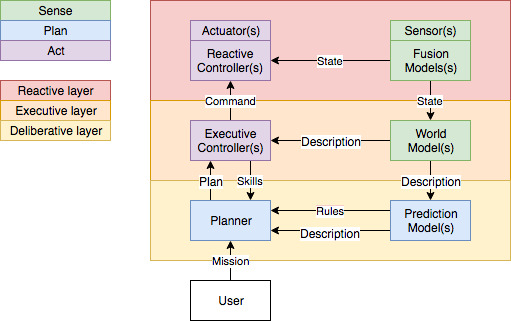
\includegraphics[scale=0.40]{img/3layers}
\end{figure}

\section{Discovery}

To collaborate, robots will need the help of the network to discover each other.
We need to discover the robots endpoints (named/addressed data streams) and the type of data exchanged.

The problem solver / planner part will also need to "understand" what kind of actions the robot can do.
The "skills" can be described with a specific language (PDDL, STRIPS, and co), and served by the robots to be downloaded by the planning part.

\section{Planning}

\subsection{Expressing the mission of a robot}
\subsection{Need to discover and get information for planning from control nodes}
\subsection{Describing the environment + control/planning loop}

\section{Control}

\subsection{Pub/Sub}

This communication pattern is used when we need the data to be sent to the consumer as fast as possible after it has bee produced.
For example, the data of a sensor that is used in a (realtime) control system.
Also, the commands of an controller that is sent to an actuator (real or virtual).

\subsection{Req/Res}

This communication pattern is used when the consumer need a big chunck of data, or data that is not updated often, or when requesting a computation task.
This can be used for example to serve the skills descriptions, where a planned will request only when the robot is discovered.
This can also be used to run some heavy computation on a server if the client is not powerful enough.

\begin{thebibliography}{1}

\bibitem{IEEEhowto:kopka}
H.~Kopka and P.~W. Daly, \emph{A Guide to \LaTeX}, 3rd~ed.\hskip 1em plus
  0.5em minus 0.4em\relax Harlow, England: Addison-Wesley, 1999.

\end{thebibliography}

\end{document}
